
\chapter{作曲に関する経緯}

\section{背景}\label{sec: background}

Beethoven以後のドイツ/オーストリアの作曲家にとって, 交響曲はBeethovenの重圧を感じずにはいられない分野であった.
その作品は形式的に完成されているだけでなく, 楽想の点でも優れており, しかも両者が高い次元で統合されている.
Beethoven没後に至って彼の作品の質の高さが周知された結果, ドイツ・オーストリア圏において「交響曲」は最も要求される水準が高い純粋器楽の最高峰とみなされることになった.
この時期に交響曲を試みた作曲家は依然として存在したが, ほとんどの作品はこの厳格な審判により批判され, 歴史の陰に消えることとなる.

19世紀中期における「交響曲の危機」は, いくつかの理由が複合して形成された複雑な社会現象であって, 実際に何が起こっていたのか解明することは難しい\cite{frisch}.
音楽の受容が18世紀には主として貴族階級で行われていたのが1830年代には教養市民階級へと移行し, そのシステムが洗練されることにより各都市に常設オーケストラが設立された.
同時にMendelssohnに始まる過去作の再演が定着することにより, 彼ら教養層は一層高度な音楽的内容を求めることになる.
その結果, Beethovenを規範とする水準の高い音楽評論が定着し, 特に交響曲に関しては極めて厳しい目が向けられることになったのである.

この状況において, すべての前期ロマン派の作曲家にとってどのような音楽を作ればよいのか, という問題に各々が自分なりの回答を出す必要に迫られることになる.
例えばFranz Lisztは交響曲というジャンルを放棄し, 新たに「交響詩」という分野を創始した.
Richard Wagnerは従来のオペラを拡大し, 自ら「楽劇」と呼称する大規模な作品を作り出した.
これらの傾向は, Beethoven以来の「絶対音楽」に対して「標題音楽」と呼ばれる新しい潮流を生み出し, 新ドイツ楽派として結実した.
それに対してSchumann路線を継承する音楽家たちも多く存在し, 両者の対立が19世紀末まで続く絶対音楽と標題音楽の激しい議論を生じさせることになる.
しかしSchumannは管弦楽分野では音楽界を牽引する作品を生み出しておらず, 絶対音楽の側に新たな旗頭が必要とされていた.

1853年にRobert Schumannの面前にJohannes Brahmsが現れたのはまさにそのような状況であった.
若きJohannesが自身のハ長調のピアノソナタを演奏し始めると, Robertは第1楽章が終わったところで隣室のClaraを呼び寄せ, 二人で全曲を改めて拝聴した.
この作品はRobertにとってBeethoven以来の伝統的様式の上に建つ新世代の理想的な芸術と感じられたに違いない.
二週間と経たずに有名な評論「新しい道」を執筆し, 新音楽時報に投稿している.
同時に, 日記において上述のソナタを「偽装された交響曲」と記し, Joachimへ宛てた手紙でJohannesが交響曲を作曲することへの期待を述べている.

その期待に応えて, Brahmsは1854年の4月には2台のピアノのためのソナタを作曲し, それを交響曲へと改作する意欲を見せている\cite{compos}.
そして実際にその第1楽章をオーケストレーションするものの, その出来栄えに満足できず, この試みは一時放棄される\footnote{なお,
この2台ピアノのためのソナタは1855年2月に見た夢が契機となりピアノ協奏曲として改作され, 1859年に初演された. 現在の作品15である.}.
こうしてBrahmsの交響曲への挑戦は1862年まで延期されることになる.


\section{作曲過程}\label{sec: process}

作品68と後にBrahms自身によって附番されたこのハ短調の交響曲は, 少なくとも1862年の夏には着想されており, ある程度作曲が進んでいた.
Brahmsの友人である作曲家のAlbert Dietrichが1862年6月にバート・クロイツナハ近郊のミュンスター・アム・シュタインに滞在中にこの第1楽章をBrahmsからピアノで聴かされている\cite{kaisouroku}.
また, Clara Schumannも同じ時期にこの楽章の楽譜をBrahmsから受け取っており, 7月1日付けのJoachimへの手紙でそのことを伝えている.
\begin{quote}
	Johannesが少し前に私に最初の交響曲の第一楽章を送ってきました. どんなに驚いたことか. それは次のように大胆に始まります.
	(譜例) %** この手紙のきちんとした出典と譜例を探す **
	それはちょっと難しいのですが, わたしはすぐに馴染みました.
	楽章は素晴らしい美しさに満ち, モティーフは巨匠的に扱われていて, ますます巨匠らしさが彼の身についてきたようです.
	すべてのものがとても興味深い方法で織り合わされています.\cite{compos}
\end{quote}
% 後に全曲の完成後, Claraは第1楽章Allegroの開始が以前のものと同じだと述べている\cite{library}.
この譜例は完成稿の第1楽章Allegroの開始 (譜例\ref{1-42}) と同じもので, 従ってこのときの第1楽章は現在の作品68の直接的な祖先となる.
一方, 前節で指摘した1854年の交響曲の試みについては, そのニ短調の第1楽章はピアノ協奏曲第1番作品15に転用されたが,
第2, 3楽章については詳細が不明で作品68に転用されたと一般に考えられているがそれを裏付ける証拠はない.
故に, 確固とした証拠に基づいて言えることは, 作品68の構想はせいぜい1876年の初演の14年前まで遡る, ということだけである.

その後, かなりの長期間に渡って交響曲の作曲の進展を伝える資料はない.
実際, 1862年時点でのBrahmsの作品リストは作品21までしか進んでおらず\footnote{ただしおおよそ作品31までは既に作曲されている.},
この慎重な作曲家が交響曲を完成させようとするには経験が不足していると考えたのも当然に思える.
\begin{quote}
	Beethovenという巨人が背後から行進してくるのを聞くと, とても交響曲を書く気にはならない.\cite{denki}
\end{quote}
という有名なBrahmsの言葉は1870年代初めにHans von Bülowに語ったものである\cite{library}.

1868年9月12日, ライン河沿いに旅行中だったBrahms\cite{compos}はClaraの誕生日にアルペンホルンの旋律
(譜例\ref{4-30}) に重ねて次のメッセージを送っている (図\ref{fig: alphorn}).
\begin{quote}
\begin{multicols}{2}
	Hoch aufm Berg, tief im Thal, \\
	grüß ich dich viel tausend mal! \\
	遥か山の高みから, 深い谷の奥底から, \\
	あなたに幾千回でも挨拶を送りましょう
\end{multicols}
\end{quote}
\begin{wrapfigure}{r}{8.0cm}
% \begin{figure}[htbp]
	\centering
    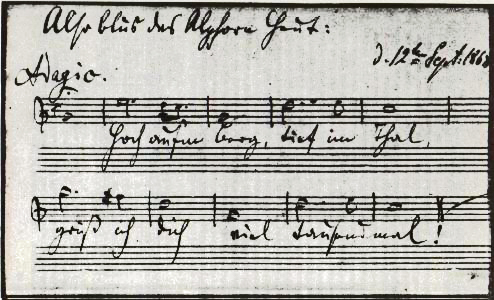
\includegraphics[clip,width=7.0cm]{./figure/alphorn.jpg}
	\caption{1868年9月, JohannesからClaraへの手紙.}
    \label{fig: alphorn}
% \end{figure}
\end{wrapfigure}

\noindent もちろんこれはハ短調交響曲の第4楽章で重要な役割を果たす旋律であるが,
しかしこの時点でBrahmsがこの旋律を自身の交響曲に用いることを考えていたかは明らかではない.
実際, 第4楽章の作曲は主として1874年に行われたとされており, この時点ではその意図はなかったと思う方が自然であろう\cite{frisch}.

1873年夏に完成したハイドンの主題による変奏曲, その年の暮れから74年頭の間に完成したピアノ四重奏曲第3番の経験を経て, Brahmsはハ短調の交響曲を完成させる気は熟したと判断したと思われる.
Simrockに「交響曲について心配は無用です. それはいずれ, われわれの出版社の名前で出されなければならないのですから」と手紙で伝える\cite{ogt}と,
%** この手紙の出典および書かれた時期を調べること もしかして76年だったりしない? \cite{library} **
1874年夏にスイスのチューリヒ湖畔リュシュリコンで第4楽章に取り組んでいる.
1875年の夏はツィーゲルハウゼンで弦楽四重奏曲第3番作品67を仕上げた\cite{compos}後に, 1876年夏のザースニッツ滞在,
そして続くハンブルク滞在中に本作に取り組み, 最終的にこの年の秋にClaraのいるバーデン・バーデン近郊のリヒテンタールで完成された (図\ref{fig: mov4-59}).
Brahmsは1876年9月に第1, 4楽章を, 10月10日には全楽章をClaraにピアノで聴かせている.
ClaraはJoachimへの手紙でこの曲を「才気に富んだ労作です」と高く評価しているものの, 旋律の活気に欠けているために「私は悲しみ,
打ちひしがれたことを隠すことができません」とも同じ手紙で述べている\cite{compos}.

\begin{figure}[htbp]
	\begin{center}
    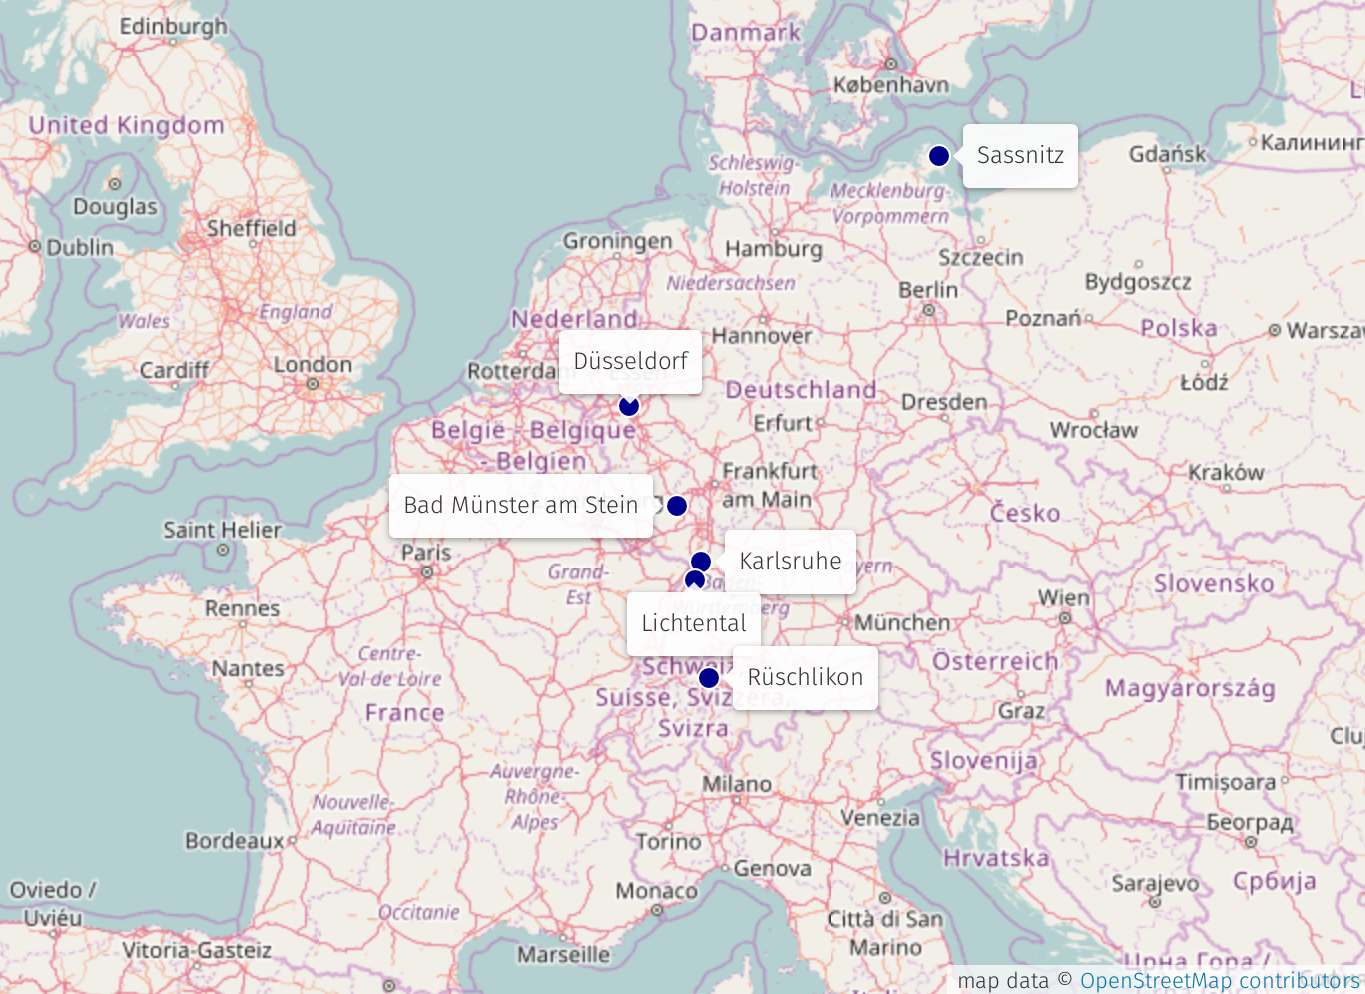
\includegraphics[clip,width=12.0cm]{./figure/map-composition.png}
	\caption{交響曲第1番が作曲された都市.
		地図はOpenStreetMapによる (\href{http://www.openstreetmap.org/copyright}{CC BY-SA}).}
    \label{fig: concert}
	\end{center}
\end{figure}


\section{初演と評価}\label{sec: premiere}

Brahmsは指揮者Otto Dessoffに楽譜を見せ, その意見をもとに改訂を加えつつ, 初演の準備を進めた.
初演は1876年11月4日, Dessoffの指揮, カールスルーエ宮廷管弦楽団の第1回予約演奏会で行われた.
それに先立つ8月13日にはバイロイト音楽祭でWagnerの「ニーベルングの指環」が初演されていることと比較すると, 優れて象徴的である.
初演の後, 半年かけてBrahmsは本作を手稿譜のまま携えて演奏旅行に出かけた (詳細な演奏データは\ref{sec: till publication}節参照).
この過程は自作の紹介とともに出版前に作品を改訂するためのもので, Brahmsはどの交響曲についてもこのプロセスを必ず綿密に遂行している.
Brahmsは常に出版稿に至るまでの途中段階の楽譜を破棄しているが, この曲に関しては,
この「試演」段階で使用されたVn1, Vn2, Vaのパート譜が完全には破棄されずに残されており, 初演時と出版時でどのような変更が加えらえたのかを窺い知ることができる.
それによると, 第2楽章は初演時には現在よりもずっと大規模で, A+B+A+C+Aという構造を取っていた.
初演稿はHenle社のスタディスコアの付録として見ることができる\cite{henle}し, Riccardo Chailly/ライプツィヒ・ゲヴァントハウス管弦楽団の2012-13年の録音などで聴くこともできる.

交響曲史上でも傑出した本作であるが, 初演は成功を収めたものの, この一連の演奏は賛否両論の激しい議論を引き起こした\cite{compos}.
特にウィーンでは演奏後に拍手が起こらなかったと伝えられる (回想録集\cite{kaisouroku}第2巻p.22-23).
これはもちろん作品自体が複雑で一聴しただけで十分に理解するのが難しいという点にも要因があるが, 何より\ref{sec: premiere}節で論じた「Beethoven問題」が大きく寄与している:
当時の評論家の問題意識は「Brahmsの新作の交響曲はBeethovenの交響曲の伝統のもとでどのように位置づけるべきか」という点に向けられていた\cite{frisch}.

coming soon


\section{出版}

完成版の楽譜がBrahmsからSimrockに発送されたのは1877年5月31日 (第2楽章を除く) で\cite{library},
1877年10月に管弦楽版総譜, パート譜, ピアノ連弾版が同時に出版されている\cite{frisch}. 出版報酬は5000ターラーであった\cite{henle}.
出版の遅れは同じ時期に交響曲第2番の作曲が進められていたことが影響していると考えられる.

出版用のスコア自筆譜は1楽章のみ1900年代初頭に失われているが, 2, 3, 4楽章はピアーポント・モーガン図書館に収蔵されている.
4楽章の終わりに"J.~Brahms Lichtenthal Sept: 76"と書き込まれている (図\ref{fig: mov4-59}) が, 当然その第2楽章はそれ以後に作成されたものである.
ピアノ連弾版自筆譜はアメリカ議会図書館に収蔵されていて, "Pörtschach Juni 77. J.~Br."と署名されている\cite{frisch}.

現在普及している楽譜は, 他の交響曲もそうだが, 1920年代のBreitkopf \& Härtel社によるBrahms全集を底本としている.
この全集版にはEusebius Mandyczewskiも加わっているが, 特に器楽曲に関してはHans Gálが編集主幹として作業に当たっている.
Dover版, あるいは国内版である音楽之友社版\cite{ogt}, 全音版はいずれもこの流れに位置づけられる.

ただ, このBH全集版は自筆譜ではなく, ウィーン楽友協会に保管されている作曲者の書き込み付き初版譜をもとにしている.
この書き込みには一時的な試し書きも含まれており, どれだけBrahmsの最終的な決定を反映しているかが微妙な問題である.
この点に注意を払ったRobert Pascall校訂による新版がHenle社から1997年に出版されている\cite{henle}.
ただしこの曲に関してはHenle版とBH全集版とでさほど重大な相違は見られない.
% むしろこの新版には破棄を免れたカールスルーエ初演時の1st, 2ndヴァイオリンとヴィオラのパート譜が付録として掲載されていることが興味深い.

なお, \href{http://imslp.org/wiki/Symphony_No.1,_Op.68_(Brahms,_Johannes)}{IMSLP}から,
管弦楽版自筆譜 (1楽章を除く), ピアノ連弾版自筆譜, Simrock社の管弦楽版初版譜, BH全集版初版譜, BH全集版パート譜などがダウンロードできる.

\begin{figure}[htbp]
	\centering
    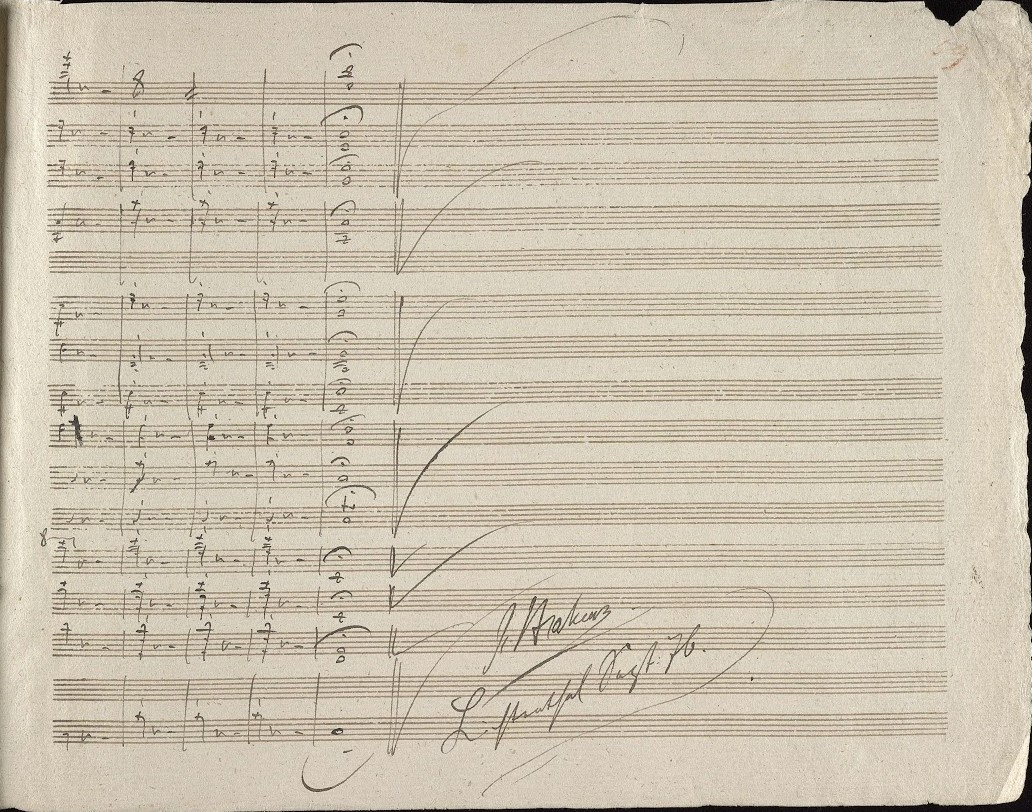
\includegraphics[clip,width=12.0cm]{./figure/mov4-59.jpg}
	\caption{自筆譜の最終ページ}
    \label{fig: mov4-59}
\end{figure}

\begin{figure}[htbp]
	\centering
    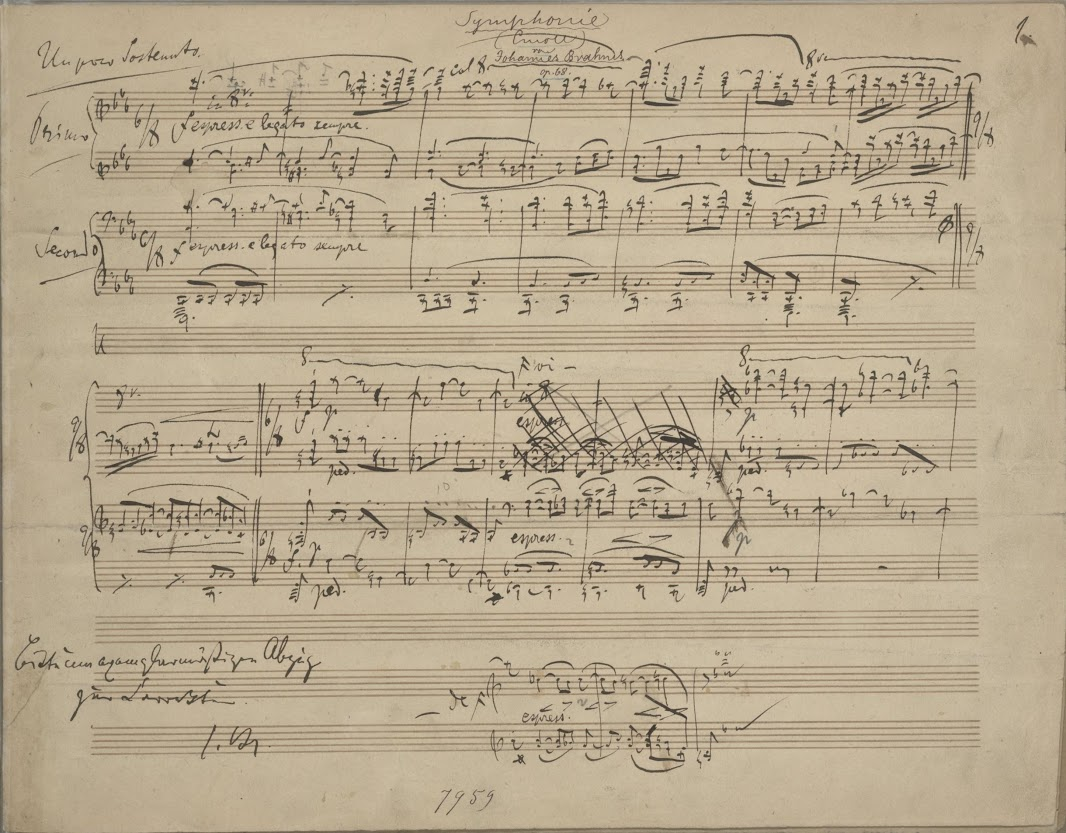
\includegraphics[clip,width=12.0cm]{./figure/mov1(4H)-01.jpg}
	\caption{ピアノ連弾版自筆譜の冒頭ページ}
    \label{fig: mov1(4H)-01}
\end{figure}
